\documentclass[letter,11pt]{article}

\usepackage[spanish,es-nodecimaldot]{babel}
\usepackage[utf8]{inputenc}

\usepackage{lmodern}
\usepackage[T1]{fontenc}
\usepackage{textcomp}

\usepackage{framed}
\usepackage[svgnames]{xcolor}
\colorlet{shadecolor}{Gainsboro!50}

\usepackage[labelfont=bf]{caption}
\usepackage{graphicx}
\usepackage{pstricks}

\usepackage{anysize}
\marginsize{3cm}{2cm}{2cm}{3cm}

\usepackage{siunitx}
\usepackage{amsmath}
\usepackage{array}
\usepackage{csquotes}

\usepackage{fancyhdr}
\usepackage{lastpage}
\pagestyle{fancy}
\fancyhf{}
\fancyhead[LE,RO]{Laboratorio de Circuitos Eléctricos I}
\fancyfoot[CO,CE]{\thepage\ de \pageref{LastPage}}

\special{papersize=215.9mm,279.4mm}

\usepackage[
    pdfauthor={Carlos Eduardo Caballero Burgoa},%
    pdftitle={Laboratorio de Circuitos Eléctricos I},%
    pdfsubject={Leyes de Kirchhoff},%
    colorlinks,%
    citecolor=black,%
    filecolor=black,%
    linkcolor=black,%
    urlcolor=black,
    breaklinks]{hyperref}
\usepackage{breakurl}

\newcommand{\blankpage}{
\newpage
\thispagestyle{empty}
\mbox{}
\newpage
}

\renewcommand{\arraystretch}{1.2}

\begin{document}

\begin{titlepage}
    \begin{center}
        {\Large UNIVERSIDAD MAYOR DE SAN SIMÓN}\\
        \vspace*{0.15cm}
        {\large FACULTAD DE CIENCIAS Y TECNOLOGÍA}\\
        \vspace*{0.10cm}
        DEPARTAMENTO DE ELÉCTRICA-ELECTRÓNICA\\
        \vspace*{3.0cm}
        {\Large \textbf{LABORATORIO DE CIRCUITOS ELÉCTRICOS I}}\\
        \vspace*{0.3cm}
        {\Large \textbf{INFORME No. 2}}\\
        \vspace*{3.5cm}
        {\Large \textbf{LEYES DE \emph{KIRCHHOFF}}}\\
    \end{center}

    \vspace*{6.4cm}
    \leftskip=7.95cm
    \noindent
    \textbf{Estudiante:}\\
    Caballero Burgoa, Carlos Eduardo.\\
    \newline
    \textbf{Carrera:}\\
    Ing. Electromecánica.\\
    \newline
    \textbf{Docente:}\\
    Ing. Marco Antonio Vallejo Camacho.\\
    \newline
    \textbf{Grupo:} 3E.\\
    \textbf{Fecha de entrega:} 16 de Abril del 2024.\\
\end{titlepage}

\section{Cálculos previos}

\begin{figure}[!h]
\centering
\includegraphics[scale=0.20]{resources/preinforme1.eps}
\end{figure}

\begin{figure}[!h]
\centering
\includegraphics[scale=0.20]{resources/preinforme2.eps}
\end{figure}

\section{Simulación}
Se utilizó el software \emph{Quite Universal Circuit Simulator.} para simular
el circuito, este puede verse en la figura (\ref{simulacion}).
\\

\begin{figure}[!h]
\centering
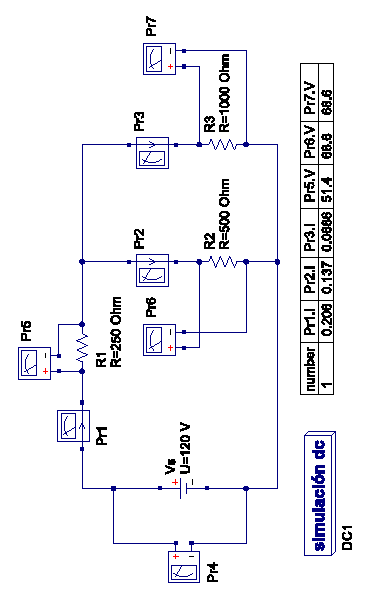
\includegraphics[scale=1.75]{resources/simulacion.eps}
\caption{Simulación de circuito.}
\label{simulacion}
\end{figure}

\newpage

\section{Tablas y mediciones}
En la figura (\ref{tablas}), se adjunta la hoja de resultados provista en la
guía de laboratorio, rellenada con la información teórica, simulada y las
mediciones realizadas en laboratorio.

\begin{figure}[!h]
\centering
\includegraphics[scale=0.20]{resources/preinforme3.eps}
\caption{Tabla de resultados.}
\label{tablas}
\end{figure}

\newpage

\section{Cuestionario}

\begin{enumerate}

\item \textbf{Aplicando las leyes de \emph{Kirchhoff} demuestre la resistencia
equivalente: (a) serie, y (b) paralelo:} \\

\begin{itemize}
    \item (a)
        \begin{figure}[!h]
        \centering
        \includegraphics[scale=1.00]{resources/figura3a.eps}
        \end{figure}

        Por ley de tensiones de \emph{Kirchhoff} se sabe que:
        \begin{equation*}
            V_{AB}=V_1+V_2+V3+\cdots+V_N
        \end{equation*}

        Usando la ley de \emph{Ohm} ($V=IR$):
        \begin{equation*}
            I_{AB}R_{AB}=I_1 R_1+I_2 R_2+I_3 R_3+\cdots+I_N R_N
        \end{equation*}

        Sabiendo que la corriente en la conexiones en serie no varia:
        \begin{equation*}
            IR_{AB}=IR_1+IR_2+IR_3+\cdots+IR_N
        \end{equation*}
        \begin{equation*}
            IR_{AB}=I(R_1+R_2+R_3+\cdots+R_N)
        \end{equation*}

        Por tanto:
        \begin{equation*}
            R_{AB}=R_1+R_2+R_3+\cdots+R_N=\sum_{n=1}^N R_n
        \end{equation*}
    \item (b)
        \begin{figure}[!h]
        \centering
        \includegraphics[scale=1.00]{resources/figura3b.eps}
        \end{figure}

        Por ley de corrientes de \emph{Kirchhoff} se sabe que:
        \begin{equation*}
            I_{CD}=I_1+I_2+I_3+\cdots+I_N
        \end{equation*}

        Usando la ley de \emph{Ohm} ($I=V/R$):
        \begin{equation*}
            \frac{V_{CD}}{R_{CD}}=\frac{V_1}{R_1}+\frac{V_2}{R_2}+
            \frac{V_3}{R_3}+\cdots+\frac{V_N}{R_N}
        \end{equation*}

        Sabiendo que el voltaje en las conexiones en paralelo no varia:
        \begin{equation*}
            \frac{V}{R_{CD}}=\frac{V}{R_1}+\frac{V}{R_2}+\frac{V}{R_3}+
            \cdots+\frac{V}{R_N}
        \end{equation*}
        \begin{equation*}
            \frac{V}{R_{CD}}=V\left(\frac{1}{R_1}+\frac{1}{R_2}+\frac{1}{R_3}+
            \cdots+\frac{1}{R_N}\right)
        \end{equation*}

        Por tanto:
        \begin{equation*}
            \frac{1}{R_{CD}}=\frac{1}{R_1}+\frac{1}{R_2}+\frac{1}{R_3}+
            \cdots+\frac{1}{R_N}=\sum_{n=1}^N\frac{1}{R_n}
        \end{equation*}
\end{itemize}

\item \textbf{(a) Aplicando la regresión lineal y los valores obtenidos y
registrados en la tabla, construya la ecuación de la curva característica
voltaje-corriente de la fuente $V_s$; (b) ¿que significado tienen los
coeficientes ``$A$'' y ``$B$'' entregados por la regresión lineal?; (c) grafique
la curva voltaje-corriente para $V_s$.}

\underline{Respuesta}:

(a) Se calcula la recta de mejor ajuste por el método de los mínimos cuadrados,
resultando los siguientes valores:

\begin{equation*}
    A = (95.49 \pm 1.02) [V]; 1.06\%
\end{equation*}
\begin{equation*}
    B = (-8.45 \pm 1.14) [\Omega]; 13.46\%
\end{equation*}

Siendo su coeficiente de correlación ($r$):

\begin{equation*}
    r = -0.9201
\end{equation*}

(b) Considerando que el modelo de ajuste es:

\begin{equation*}
    V_0 = V_s - R_s I_0
\end{equation*}

$A$ representa el valor $V_s$ es decir, el voltaje medido en las terminales de
la fuente en circuito abierto, sin carga.

$B$ representa el valor de $R_s$, es decir, la resistencia interna de la fuente
de tensión.

\begin{center}
\begin{tabular}{|>{\centering}m{9.2cm}<{\centering}|}
\hline
\textbf{Resultado}
\tabularnewline \hline
$V_s = (95.49 \pm 1.02) [V]; 1.06\%$ \tabularnewline
$R_s = (8.45 \pm 1.14) [\Omega]; 13.46\%$ \tabularnewline
\hline
\end{tabular}
\end{center}
\vspace{0.10cm}

A partir de los datos obtenidos se genera la gráfica en la
\textbf{Figura~\ref{figura}}.

\begin{figure}[!h]
\centering
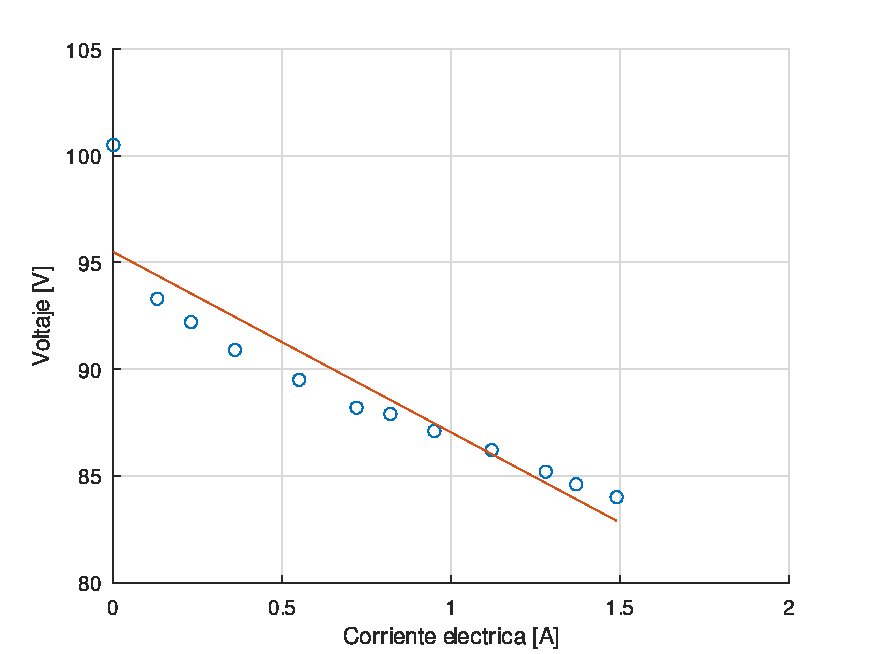
\includegraphics[width=0.85\textwidth]{resources/o1.eps}
\caption{Gráfica de corriente vs voltaje.}
\label{figura}
\end{figure}

\item \textbf{(a) ¿Cual es el voltaje de regulación para una fuente ideal?; (b)
¿cual es el voltaje de regulación de la fuente $V_s$ empleada en esta practica
de laboratorio?}\\

Considerando:
\begin{equation*}
    \%_{\text{regulación}} = \frac{V_{SL}-V_{FL}}{V_{FL}}\,100 \%
\end{equation*}

Donde:
\begin{itemize}
    \item $V_{SL}$: Voltaje sin carga.
    \item $V_{FL}$: Voltaje con carga completa.
\end{itemize}
\vspace{0.20cm}

(a) En una fuente ideal:
\begin{equation*}
    V_{SL} = 100 [V]
\end{equation*}
\begin{equation*}
    V_{FL} = 100 [V]
\end{equation*}

Por tanto:
\begin{equation*}
    \%_{\text{regulación}} = \frac{100-100}{100}\,100 = 0 \%
\end{equation*}
\vspace{0.20cm}

(b) En la fuente medida:
\begin{equation*}
    V_{SL} = 100.5 [V]
\end{equation*}
\begin{equation*}
    V_{FL} = 84.0 [V]
\end{equation*}

Por tanto:
\begin{equation*}
    \%_{\text{regulación}} = \frac{100.5-84.0}{84.0}\,100 = 19.64 \%
\end{equation*}
\end{enumerate}

\section{Conclusiones}
Se demostró que tanto la ley de corrientes, como la ley de tensiones de
\emph{Kirchhoff} se cumplen de modo experimental.

También se pudo apreciar la caída de voltaje respecto a la cantidad de corriente
eléctrica que fluye en un circuito, pudiendo apreciarse claramente la curva
característica voltaje-corriente.

\end{document}

